\raggedright
\section{Profiling}

texto
\newline

\subsection{Education}
Variable Type: Categorical Nominal.\newline
Recall: the Education variable describes the level of studies the consumer has (2nd cycle, Basic, Graduation, Master, PhD).

\begin{figure}[H]
    \centering
    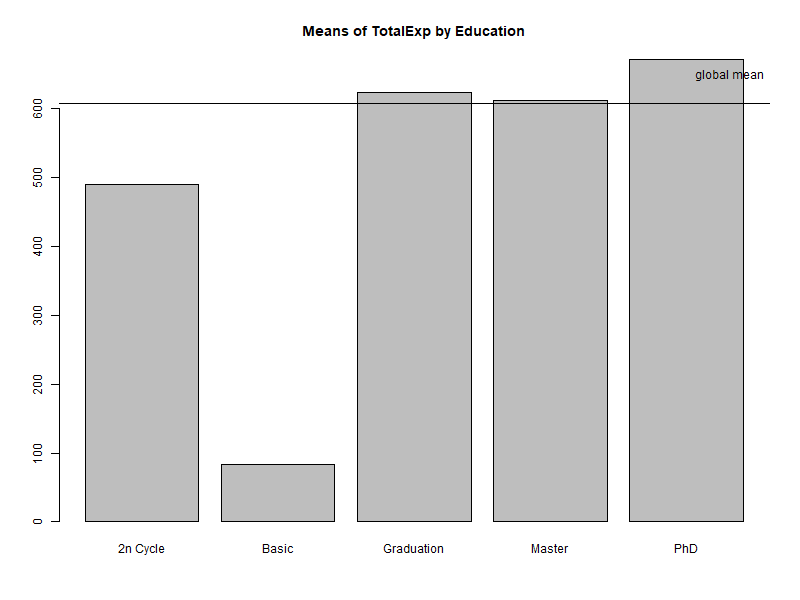
\includegraphics[width=0.8\linewidth]{Imatges/mean_barplot_TotalExp.png}
    \caption{Descripció}
    \label{fig:scree_plot}
\end{figure}
\newline
With a mean barplot we can see the total expent depending on the level of studies, where it is evident that the basic education group spends much less money on their purchase.


\begin{figure}[H]
    \centering
    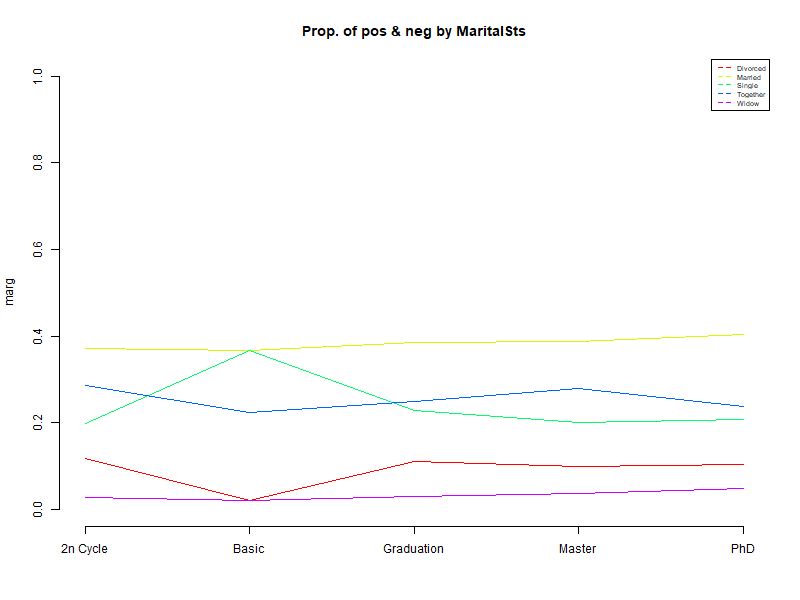
\includegraphics[width=0.8\linewidth]{Imatges/prop_cond_class_MaritalSts_4_legend.png}
    \caption{Descripció}
    \label{fig:scree_plot}
\end{figure}
\newline
Comparing with the marital status we can see that independently of their studies, the customers usualy are married or together. It is worth noting that those with a basic education level are more often married or single.
\begin{figure}[H]
    \centering
    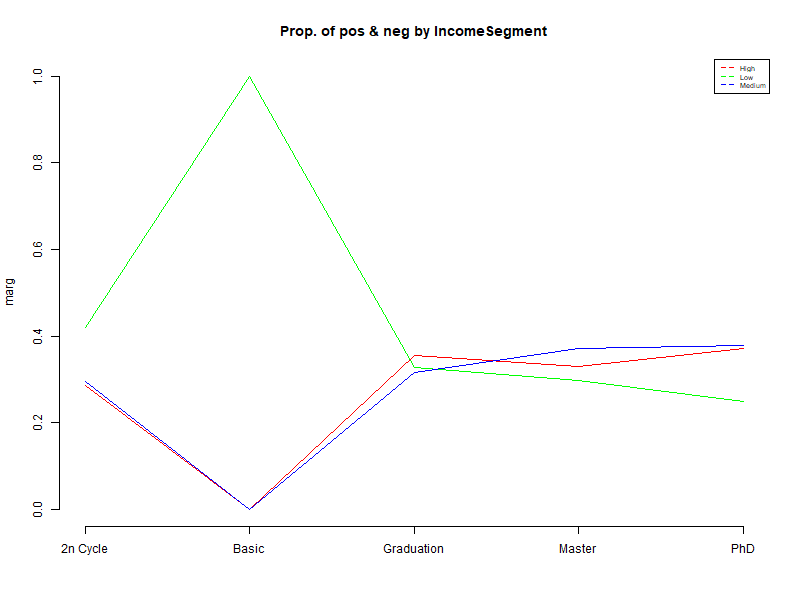
\includegraphics[width=0.8\linewidth]{Imatges/prop_cond_class_IncomeSegment_4_legend.png}
    \caption{Descripció}
    \label{fig:scree_plot}
\end{figure}
\newline
Comparing the income segment we can see that the basic level has the highest frequency with low segment. It shows that they are the ones with the lowest incomes, followed by those with a second-level education, and that there is not much difference among the rest.
\begin{figure}[H]
    \centering
    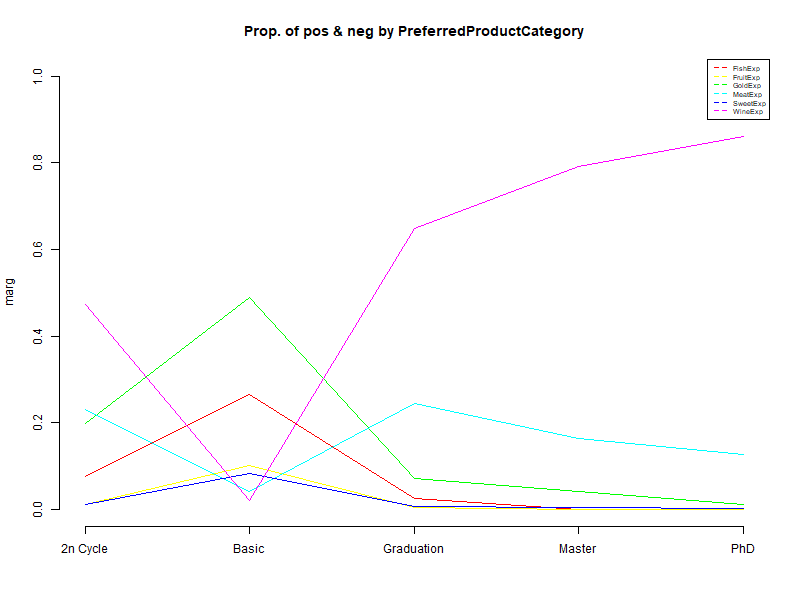
\includegraphics[width=0.8\linewidth]{Imatges/prop_cond_class_PreferredProductCategory_4_legend.png}
    \caption{Descripció}
    \label{fig:scree_plot}
\end{figure}
\newline
About their most purchased product category, we can see that as the level of education increases, there is a tendency to spend more on wine, the customers with lower education levels prefer to buy gold, and those with a graduation level education tend to spend on meat.
\subsection{MaritalSts}
Variable Type: Categorical Nominal.\newline
Recall: the MaritalSts variable describes the marital status of the customer (Divorced, Married, Single, Together, Widow).
\subsection{Kidhome}
Variable Type: Numerical Discrete.\newline
Recall: the Kidhome variable describes the number of small children in the customer's household (0 - 5).
\subsection{Teenhome}
Variable Type: Numerical Discrete.\newline
Recall: the Teenhome variable describes the number of teenagers in the customer's household (0 - 5).
\subsection{Response}
Variable Type: Categorical Binary.\newline
Recall: the Response variable describes whether the customer accepted the offer in the last campaign (0 or 1).
\subsection{Complain}
Variable Type: Categorical Binary.\newline
Recall: the Complain variable describes whether the customer has filed a complaint in the last 2 years (0 or 1).
\subsection{HasChildren}
Variable Type: Categorical Binary.\newline
Recall: the HasChildren variable  whether the customer has children or not (0 or 1).

\subsection{PrefereredChannel}
Variable Type: Categorical Nominal.\newline
Recall: the PrefereredChannel variable describes the channel with highest frequency.
\subsection{PrefereredProductCategory}
Variable Type: Categorical Nominal.\newline
Recall: the PrefereredProductCategory variable describes the channel with highest frequency.
\subsection{AccCmp1}
Variable Type: Numerical Discrete.\newline
Recall: 
\subsection{AccCmp2}
Variable Type: Numerical Discrete.\newline
Recall: 
\subsection{AccCmp3}
Variable Type: Numerical Discrete.\newline
Recall: 
\subsection{AccCmp4}
Variable Type: Numerical Discrete.\newline
Recall: 
\subsection{AccCmp5}
Variable Type: Numerical Discrete.\newline
Recall: 
